% Notes on the writing of the Master Thesis
% Book: How to Write a Lot, Paul Silvia, 2nd Edition
% Book: Getting Things Done, David Allen
%
%
% Mögliche Abgrenzung von anderen: Den hybriden Ansatz von SBST mit DSE verwenden, 
% so wie im Paper von Baars et al.
%
% Mögliche weitere Evaluation: Vergleiche die Coverage von generierten Tests zu der 
% Coverage von manuell geschriebenen Tests von Entwicklern in evaluierten Programmen.
% 

\documentclass{article}
% Please do not change this options...
\usepackage[a4paper, total={6in, 10in}]{geometry}
\usepackage{graphicx}
\graphicspath{ {./img/} }
\usepackage{todonotes}
\usepackage{acronym}
\usepackage{algorithm}
\usepackage{amsmath}
\usepackage{algpseudocode}
\algblock{Input}{EndInput}
\algnotext{EndInput}
\algblock{Output}{EndOutput}
\algnotext{EndOutput}
\newcommand{\Desc}[2]{\State \makebox[2em][l]{#1}#2}
\usepackage[T1]{fontenc}
\makeatletter
\newcommand\BeraMonottfamily{%
  \def\fvm@Scale{0.85}% scales the font down
  \fontfamily{fvm}\selectfont% selects the Bera Mono font
}
\makeatother


\usepackage{listings}
\lstset{
  numbers=left,
  xleftmargin=2.5em,
  framexleftmargin=2.5em,
  frame=tb,
  stepnumber=1,    
  firstnumber=1,
  numberfirstline=true,
  basicstyle=\BeraMonottfamily,
  identifierstyle=,
  stringstyle=\ttfamily,
  %keywordstyle=\color{OliveGreen},
  keywordstyle=,
  showstringspaces=false
}

% This package must be declared last
\usepackage{cleveref}

\begin{document}

\title{Master Thesis}
\author{Vsevolod Tymofyeyev}
\date{\today}
\maketitle

\tableofcontents
\newpage
\section{Introduction}
In der Programiersprachenwelt, in der es zwei große Fronten gibt (low-level Sprachen, die auf Kosten von Sicherheit mehr Performanz bieten und high-level Sprachen, die durch bestimmte Konstrukte wie Garbage-Collector Sicherheiten für Programmierer bieten, die jedoch zu Laufzeit-Overhead führen) versucht Rust beides zu verbinden. Die statisch typisierte Sprache für Systemprogrammierung verspricht eine ähnlich hohe Performanz wie C++ mit erweiterter Typ- und Speichersicherheit by default. Invarianten werden zur Kompilierzeit sichergestellt, wodurch Abstraktionen (sogenannte Zero-Cost-Abstractions) und automatische Speicherverwaltung mit keinen Laufzeitkosten verbunden sind, wie es zum Beispiel bei Sprachen mit Garbage Collection der Fall ist. Rust verhindert unter anderem folgende oft verbreitete Probleme: 
\begin{itemize}
    \item Dangling pointers
    \item Data races
    \item Integer overflow
    \item Buffer overflow
    \item Iterator invalidation
\end{itemize}
Nur die Integer und  Buffer overflows werden zur Laufzeit überprüft, wobei die Buffer overflows durch das Benutzen von Iteratoren auf statische Checks reduziert werden können~\cite{Anderson2016}. Diese Symbiose führte dazu, dass die Sprache besonders attraktiv auf Entwickler wirkt, wodurch sie trotz ihres sehr jungen Geschichte bereits seit mehreren Jahren die Beliebtheitsrankings stürmt~\cite{StackOverflow2020}. Selbst Spitzenkonzerne erwägen die Anwendung von Rust in Teilen ihrer Software. Laut Microsoft und Google sind 70\% der in ihrer Software in den vergangenen Jahren gefundenen Fehler auf Speicherlecks zurückzuführen, hervorgerufen durch die weitverwendeten unsicheren Sprachen wie C und C++~\cite{Microsoft2019MemoryBugs, RustInAndroid}. Microsoft, SpaceX, Google, Amazon AWS und viele andere Unternehmen fingen bereits an, Rust in ihren Produkten zur erhöhten Sicherheit zu verwenden~\cite{MicrosoftJoinsRust, AmazonLovesRust, RustInAndroid, GoogleRustFoundation}.

Nichtsdestotrotz, kann auch der Rust Compiler nicht die komplette Korrektheit eines Programms garantieren, wodurch auch bei der Programmierung mit dieser Sprache das Testen der geschriebenen Software einem nicht erspart bleibt. Software Testen erfodert Daten, deren manuelle Selektion die Aufgabe eines Programmierers ist. Dieses Vorgehen ist aber in der Regel sehr aufwändig und kostenintensiv. Eine genügend komplexe Software kann Tausende Ausführungspfade haben, die durch verschiedene Inputdaten angesteuert werden und von einem Menschen unter Umständen übersehen werden können, schließlich müssten fast genauso viele Tests geschrieben werden. Ein weiterer Punkt ist, dass sich Software-Anforderungen mit der Zeit ändern können, was dazu führt, dass existierende Testsuites dadurch eventuell manuell verändert bzw. im schlimmsten Fall neu geschrieben werden müssen. Somit ist das Abdecken von allen möglichen Ausführungsfällen oder gar eine exhaustive Coverage schlicht wirtschaftlich und menschlich kaum zu leisten~\cite{Myers2012}. Es wird angenommen, dass ungefähr die Hälfte des Budgets in Software Projekten für das Testen ausgegeben wird. Es ist also nicht überraschend, dass ungefähr~\cite{Harman2015}. Außerdem, trotz der ausgereiften Testing Tools, stehen Entwickler oft unter Zeitdruck (z. B. Deadlines bei Projekten) und haben nicht genug Zeit, die immer komplexer werdende Software zu testen. Das ist ein großes Problem, denn auch wenn einige kleinen Bugs nur zur Unzufriedenheit eines Endnutzers führen, können einige andere erhebliche wirtschaftliche und selbst gesundheitliche Schäden auslösen~\cite{Myers2012}. \todo{Ein paar Beispiele für krasse Vorfälle wegen Software Bugs wären hier praktisch, z. B. Arianne V Explosion} Aus diesem Grund sind in den letzten Jahren bzw. Jahrzehnten viele Ansätze entstanden, um diesen Prozess zu automatisieren, indem Tests aus einer gegebenen Software generiert werden~\cite{McMinn_2004}. 

Da Rust als stabile Programmiersprache als jung gilt und im Jahr 2015 in der Version 1.0 erschien~\cite{Rust10}, gibt es zum Stand des Schreibens nur relativ wenige Optionen für eine automatische Testgenerierung. Diese beschränken sich auf Tools, die mittels Symbolic Execution die möglichen Pfade in einem gegebenen Programm durchsuchen~\cite{cadar2008klee}. \todo{Weitere Tools?} Außerdem benutzen die Tools die IR von LLVM, welches vom Rust Compiler eingesetzt wird. Zusätzlich bringt das affine Typ-System von Rust~\cite{Anderson2016} einige Hürden mit, verglichen zu Sprachen wie z. B. Java. Es gibt aber zum Stand des Schreibens keinen bekannten Einsatz von SBST für Rust. SBST ist eine Kombination aus automatischer Testgenerierung und metaheuristischen Suchtechniken. Diese Unterkategorie von SBSE greift zu Optimisierungsalgorithmen, um ein eigentlich NP-hartes Problem der Testgenerierung mit möglichst hoher Testabdeckung möglichst effizient und effektiv zu lösen~\cite{Khari2019}. SBST optimizes a solution as much as possible with respect to a certain objective, which could be test case priorization, test suite minimization, max out real-time properites of the SUT, and so on~\cite{Khari2019}. Die dadurch generierten Tests streben eine höhere Coverage an, um möglichst viele Fälle abzudecken. 

\section{Background}
\subsection{Test Generation in General}
\todo{Structural, functional, etc. testing}
Testsgenerierung ist ein aktiv erforschtes Feld in der Wissenschaft. Im Idealfall kann für ein Programm eine Testsuite von Unit Tests generiert werden, die alle möglichen Pfade im \ac{SUT} abdecken und gleichzeitig die Korrektheit der Ausführung jedes einzelnen Pfades durch automatische Orakel überprüft, beispielsweise durch Assertions. Ein Orakel ist ein Mechanismus zum Überprüfen, ob ein Output bei einem gegebenen Input richtig ist, beispielsweise mit Hilfe einer formalen Spezifikation~\cite{10.1145/1569901.1570127}. Leider ist das oft nicht möglich. Zum einen können in einem Programm Ausführungspfade existieren, die schlicht unter keinen Umständen erreicht werden können. Zum anderen hat Software nur sehr selten eine formale Spezifikation, die bei der Generierung verwendet werden kann, um Orakel zu generieren. Somit muss in den meisten Fällen ein Entwickler bzw. Tester die generierte Testsuite manuell mit Orakeln versehen (dazu muss er/sie natürlich selbst wissen was das richtige Verhalten ist)~\cite{Fraser_2013}. Dazu muss die generierte Testsuite aber auch möglichst klein und für den Menschen verständlich gehalten werden. 

Bei einer Testgenerierung wird das Coverage-Kriterium oft als eine Leitlinie benutzt~\cite{Fraser_2011}. Ein Coverage-Kriterium ist eine Sammlung von Test-Zielen, die typischerweise eins nach dem anderen abgearbeitet bzw. abgedeckt werden, wobei die notwendigen Input-Daten beispielsweise symbolisch oder such-basiert ermittelt werden. Eine beliebte Art des Coverage-Kriteriums ist die Branch-Coverage. 

Branches sind z. B. Arme einer if-Verzweigung oder eines Schleifenkopfes. Diese werden dann ausgeführt, wenn ein bestimmter boolischer Ausdruck zu \lstinline{true} bzw. \lstinline{false} evaluiert. Branches können auch verschachtelt sein, und um passende Werte zu finden, um einen (verschachtelten) Branch zu erreichen, kann symbolic execution bzw. seine dynamische Erweiterung mit konkreten Werten verwendet werden. Dabei wird ein Pfad aufgebaut, der mit einem \ac{SMT}-Solver nach konkreten Werten (falls solche existieren und der Pfad überhaupt erreichbar ist) aufgelöst werden kann. Eine Alternative zur symbolischen Ausführung ist eine meta-heuristische Suche. Fraser und Arcuri~\cite{Fraser_2011} listen ein paar verwante Paper dazu auf. 

\subsection{Automatically Generated Oracles}
\label{sec:generated-oracles}
Davis and Weyuker~\cite{10.1145/800175.809889} haben den Begriff non-testable programs einfegührt, der solche Programme einschließt, für die es keinen Testorakel gibt oder ein Testorakel praktisch nicht umsetzbar ist, und man somit das Ergebnis der Berechnung nicht auf Korrektheit überprüfen kann. Dazu gehören Programme, die entweder erstellt wurden, um das Ergbenis überhaupt zu erfahren, oder Programme, die zu viele Ergebnisse liefern, um sie alle zu überprüfen, oder der Entwickler hatte die Spezifikation missverstanden. Um das Problem eines fehlenden Orakels zu lösen, führten die Autoren einen sogenannten Pseudoorakel ein. Ein Pseudoorakel ist ein zweites, unabhängig implementiertes Programm, das derselben Spezifikation entsprechen muss. Es ist wichtig, dass die zwei Programme von separaten Teams ohne Zwischenkommunikation erstellt werden, damit keine Missverständnisse von einem in das andere Team propagieren können. Anschließend können die Ergebnisse der Berechnungen des originalen Programms und des Pseudoorakels verglichen und es kann über die Validität entschieden werden. 

Das manuelle Erstellen von Pseudoorakeln ist sehr mühselig und ist im Kontext von Testgenerierung für große Projekte nicht lohnenswert. Harman et al.~\cite{1265732} haben das Prinzip der Testability Transformations vorgestellt. Diese sind Quelltext-zu-Quelltext Transformationen, die zum Verbessern der Performanz verschiedener Testgenerierungstechniken führen sollen. McMinn~\cite{10.1145/1569901.1570127} hat diese Idee aufgegriffen und vorgeschlagen, Pseudoorakel für ein gegebenes Programm automatish zu generieren. Er wendet Testability Transformations an, um das originale Programm zu verändern und eine zweite Version zu generieren, die scheinbar gleiche Ausgaben wie die originale haben sollte, es jedoch zu Diskrepanzen kommen kann. Dazu hat er zwei Beispiele aufgeführt: Fließkomma-Arithmetik und Multithreading in Java. Beim Ersteren werden, beispielsweise Additionen zwischen primitiven Fließkommatypen, die nach dem IEEE-Standard etwas ungenau in den hinteren Nachkommastellen sind~\cite{10.1145/103162.103163}, durch Javas BigDecimal vertauscht. Zum Beispiel führt die Berechnung~$0.1 + 0.1 + 0.1$ in Java zum Ergebnis~$0.30000000000000004$, anstatt~$0.3$ (siehe~\cref{lst:java-transformations}).

\begin{lstlisting}[language=Java, caption=Comparing floating-point arithmetic in Java using double compared to BigDecimal~\cite{10.1145/1569901.1570127}, label=lst:java-transformations]
System.out.println(0.1 + 0.1 + 0.1);
// Ausgabe: 0.30000000000000004

System.out.println(
    new BigDecimal("0.1").add(
        new BigDecimal("0.1").add(
            new BigDecimal("0.1")
        )
    )
);
// Ausgabe: 0.3
\end{lstlisting}
In einem anderen Beispiel wendet McMinn Transformationen zum Serialisieren/Deserialisieren eines Multithreading-Programm. Dabei werden Methoden einer Klasse mit Javas \lstinline{synchronize} versehen bzw. das Schlüsselwort wird bei bereits synchronisierten Methoden entfernt. \lstinline{synchronize} sorgt dafür, dass nur ein Thread gleichzeitig die jeweilige Methode verwenden darf. In der Evaluation versucht der Autor, die durch Transformationen generierten Orakel mit Hilfe für eine genetisch-basierte Suche nach Input-Daten zu verwenden, die die Diskrepanz zwischen den Ausgaben eines originalen Programms und seines Psudoorakels maximieren. Damit können nicht nur potenzielle Bugs automatisch entdeckt (Diskrepanz), sondern auch ihr Schweregrad gemessen (Größe der Diskrepanz) werden. Die Idee von automataisch generierten Pseudoorakel wurde auch von Fraser und Arkuri~\cite{Fraser_2013} aufgegriffen. \todo{Da fehlt was}

\subsection{Random Search}
Random Search ist eine Baseline Strategie, die nicht auf Rekombination, Mutation oder Selektion zurückgreift, sondern auf Ersetzen von bestehenden Lösungen setzt. Die Idee ist, immer wieder neue Lösungen aus dem Suchraum nach dem Zufallsprinzip zu sampeln, wobei eine vorige Lösung durch die neue ersetzt wird, falls der Fitnesswert der neuen Lösung besser ist. Random Search kann von einem Archiv Gebrauch machen, indem eine Samplingstrategie wie \todo{Samplingstrategie beschreiben} eingesetzt wird~\cite{Campos2017}.

Random Testing ist eine Variante von Random Search, die Test Suites inkrementell aufbaut. Mit Random Testing wird das Programm mit zufälligen Eingaben ausgeführt und die ausgeführten Strukturen des Programms werden beobachtet. Einzelne Test Cases werden aus dem Suchraum gesampelt, und falls ein Test Case die gesamte Coverage der Testsuite erhöht, wird er behalten und ansonsten verworfen~\cite{Campos2017}. Da die Landschaft der Fitnesswerte bei der Generierung von Unit Tests ziemlich flach ist und das ein relativ simples Suchproblem ist, kann Random Search mindestens genauso effektiv sein wie evolutionäre Algorithmen und manchmal sogar besser~\cite{Shamshiri2015a}. 

\subsection{Symbolic Execution}
Symbolische Ausführung ist keine Ausführung des Programms in direktem Sinne. Vielmehr ist das ein Prozess, bei dem Programmvariablen symbolische Ausdrücke zugewiesen werden, während ein Pfad in der Programmstruktur verfolgt wird~\cite{McMinn_2004}. So ein Pfad kann aus mehreren Einschränkungen bestehen. Symbolische Ausführung ist ein verbreiteter Ansatz, um Inputdaten oder ganze Unit-Tests zu generieren, indem die Pfadeinschränkungen aufgelöst werden. \todo{Werke über DS referenzieren} Grundsätzlich folgen alle Tools dem gleichen Prinzip: Statt Programme mit manuellen oder generierten Inputdaten laufen zu lassen, werden Inputdaten mit symbolischen Werten besetzt, die initial ''alles'' sein können~\cite{cadar2008klee}. Konkrete Operationen auf Daten werden durch solchen ersetzt, die die symbolischen Daten manipulieren können. Wenn sich die Ausführung des Programms verzweigt, behalten die Tools die Ausführung beider Branches ''im Auge''. Für jeden Branch wird eine Sammlung von Einschränkungen (Constraints) gespeichert, die für die Ausführung des jeweiligen Pfades gelten müssen. Wenn die Ausführung in einem Pfad endet oder das Programm abstürzt, kann daraus ein Test generiert werden, indem konkrete Werte als Inputdaten eingesetzt werden, die die entsprechenden Pfad-Constraints erfüllen. Wenn das Programm deterministisch und unverändert bleibt, führt eine Ausführung mit konkreten Inputdaten zum selbem Bug im Program. 

Dynamische symbolische Ausführung ist eine Erweiterung von DS, die erlaubt, mit Hilfe einer Kombination aus konkreten und symbolischen Werten eine Reihe von Problemen zu überwinden~\cite{Fraser_2013}.

\subsection{Evolutionary algorithms}
Der potenzielle Suchraum für mögliche Inputdaten selbst bei einem sehr simplen Programm kann unendlich groß sein. Metaheuristische Ansätze versprechen eine Abhilfe. Das sind keine geschlossenen Algorithmen an sich, sondern Strategien, die auf spezifische Probleme angepasst werden können. Für die Generierung von Testdaten wird eine problem-spezifische Fitnessfunktion definiert, mit deren Hilfe die Qualität möglicher Lösungen des Problems verglichen werden kann~\cite{McMinn_2004}. Metaheurische Suche wird nicht nur für Testdatengenerierung verwendet. Andere Verwendungen umfassen:
\begin{itemize}
	\item Coverage der Programmstruktur als Teil einer White-Box Teststrategie,
	\item das Auswerten eines spezifischen Programmfeatures nach seiner formalen Spezifikation,
	\item Versuche, automatisch Fehlerbedingungen oder Brüche von Assertions in einem Programm herbeizurufen
	\item Verifizierung nicht-funktionaler Features, beispielsweise worst-case Ausführungszeit eines Programmteils finden.
\end{itemize}
Evolutionary algorithms setzen auf simulierte Evolution bei der Suche nach Lösungen zu einem spezifischen Problem und evolvieren Lösungskandidaten mit Hilfe von speziellen Operatoren, die von Genetik und natürlicher Selektion inspiriert sind. Genetische Algorithmen sind die bekannteste Ausprägung der evolutionären Algorithmen und nehmen ihre Anfänge irgendwo her. \todo{Keine Ahnung, ob das überhaupt sinnvoll ist, die Geschichte davon aufzuschreiben.} Eine Suche mit genetischen Algorithmen wird auf Basis von Rekombination von Zwischenlösungen durchgeführt, einem Mechanismus, um Informationen zwischen Lösungen auszutauschen und somit neue züchten~\cite{McMinn_2004}.

\subsubsection{Genetic Algorithms}
McMinn hat ein super Beschreibung von genetischen und evolutionären Algorithmen, Selektion, Crossover, Mutation, fortgeschrittene Repräsentationen von Individuen~\cite{McMinn_2004}. Außerdem wird der genetische Algorithmus in \cite{Fraser2011} und \cite{Fraser_2013} beschrieben. \cite{Fraser_2013} beschreibt außerdem die Suchoperatoren. 

In seinem Paper beschreibt Harman~\cite{Harman2002}, wie bestimmte Variablen innerhalb von Verzweigungsknoten bei der Suche rausgefiltert werden können, weil sie keinen Einfluss auf die Branch Distance haben. Somit wird der Suchraum verkleinert. 

Genetische Algorithmen sind die meist verbreitete Form von evolutionären Algorithmen, da sie einfach zu implementieren sind und im Schnitt gute Ergebnisse erzielen. Der Name ''genetischer Algorithmus'' kommt von der Analogie zwischen dem Enkodieren eines Lösungskandidaten als eine Sequenz von simplen Komponenten und der genetischen Struktur eines Chromosomes. Diese Analogie wird fortgeführt, indem einzelne Lösungen als Individuen oder Chromosomen bezeichnet werden~\cite{Campos2017}. Demnach werden Komponenten einer Lösung Gene genannt, wobei mögliche Werte einer Komponente Alleles und ihre Position in der Sequenz Locus heißen. Des Weiteren wird eine tatsächliche enkodierte Repräsentation einer Lösung, die von einem genetischen Algorithmus manipuliert wird, Genotyp und eine dekodierte - Phenotyp genannt~\cite{McMinn_2004}. Algorithm \labelcref{alg:genetic-algorithm} zeigt abstrakt die Funktionsweise eines Standard genetischen Algorithmus. Die initiale Population wird typischerweise zufällig generiert oder aus einem bestimmten Seed generiert. In folgenden Generationen werden Nachkommen mittels Optimisierungs- oder Suchoperatoren gezüchtet, also Rekombination und Mutation. Es gibt viele Variationen des Standard GA. Zum Beispiel werden bei der monotonen Variante des Standard GA nach der Mutation und Evaluation der Fitness der Nachkommen entweder die besten Nachkommen oder die besten ''Parents'' der nächsten Population hinzugefügt. Beim Standard GA werden an der Stelle sowohl ''Parents'' als auch Nachkommen der nächsten Population hinzugefügt. Eine weitere Variante von Standard GA ist der Steady State GA, der wie die monotone Variante nur die besten Individuen nach einer Mutation behält, jedoch anstatt eine neue Population von Nachkommen zu kreieren, ersetzt die ''Parents'' durch Nachkommen in der ursprünglichen Population~\cite{Campos2017}.

Die Selektion von Individuen wird durch Fitness Funktionen gesteuert, sodass Individuen mit guter Fitness mit höher Wahrscheinlichkeit überleben und in der Zucht von Nachkommen teilnehmen. Im Kontext von Testgenerierung basieren Fitness Funktionen auf Kriterien der Code Coverage, wie z. B. Statement oder Branch Coverage. In den letzten Jahren gab es einen Trend, die Suche nach mehreren Coverage Kriterien gleichzeitig zu optimieren. Da Coverage Kriterien typischerweise keine widersprüchliche Ziele darstellen, können diese in einer weigted linearen Funktion kombiniert werden~\cite{Rojas2015}. Eine hohe Anzahl von Coverage Zielen kann jedoch die Performanz eines evolutionären Algorithmus negativ beeinflussen. Um das zu vermeiden, können generierte Tests für abgedeckte Ziele in einem Archiv gespeichert werden~\cite{Rojas2017}, wobei die Fitness Funktion dynamisch adaptiert wird, um die Suche nur in Richtung nicht abgedeckter Ziele zu leiten. Der Archiv kann auch bei für bessere Effektivität von Suchoperatoren verwendet werden, in dem beispielsweise neue Tests durch Mutation von bestehenden aus dem Archiv und nicht zufällig generiert werden~\cite{Campos2017}. 
\begin{algorithm}
\caption{A high level description of a standard genetic algorithm~\cite{Campos2017}}\label{alg:genetic-algorithm}
\begin{algorithmic}
\Input
  \Desc{$C$}{Stopping condition}
  \Desc{$\delta$}{Fitness function}
  \Desc{$p_s$}{Population size}
  \Desc{$s_f$}{Selection function}
  \Desc{$c_f$}{Crossover function}
  \Desc{$c_p$}{Crossover probability}
  \Desc{$m_f$}{Mutation probability}
  \EndInput
  \Output
  \Desc{$P$}{Population of optimized individuals}
  \EndOutput
\State $P \gets GenerateRandomPopulation(p_s)$
\State $PerformFitnessEvaluation(\delta, P)$

\While{$\neg C$}
    \State $N_P \gets \{\}$
    \While{$\left| N_P \right| < p_s$}
        \State $p_1, p_2 \gets Selection(s_f, P)$
        \State $o_1, o_2 \gets Crossover(c_s, c_p, p_1, p_2)$
        \State $Mutation(m_f, m_p, o_1)$
        \State $Mutation(m_f, m_p, o_2)$
        \State $N_P \gets N_P \cup \{o_1, o_2\}$
    \EndWhile
    \State $P \gets N_P$
    \State $PerformFitnessEvaluation(\delta, P)$
\EndWhile
\State \Return $P$
\end{algorithmic}
\end{algorithm}

\subsubsection{Crossover}
Ein wesentlicher Teil von genetischen Algorithmen ist die sogenannte Rekombination oder auch Crossover. Dieser Operator nimmt zwei Parent-Lösungen als Input und verbindet sie in einer bestimmten Weise, um zwei Nachkommen-Lösungen zu produzieren. Es gibt viele verschiedene Arten von Rekombination, aber die einfachste ist die One-Point-Rekombination~\cite{McMinn_2004}. Dabei wird ein einzelner Punkt in den zwei Lösungssequenzen gewählt, der die Sequenzen in Kopf und Schwanz trennt. Die Köpfe bzw. die Schwänze werden dann zwischen den beiden Sequenzen ausgetauscht. Eine One-Point Rekombination von zwei Individuen $[0, 255, 0]$ und $[255, 0, 255]$, die in Binärform jeweils als $000000001111111100000000$ und $111111110000000011111111$ enkodiert wären, an der Stelle $12$ würde zu folgenden zwei Nachkommen führen~\cite{McMinn_2004}:
\[
\left.\begin{array}{c}
000000001111 \\  %  
111111110000 % 
\end{array}\right| 
\begin{array}{c}
111100000000 \\  %  
000011111111 % 
\end{array} \longrightarrow
\begin{array}{c}
000000001111000011111111 \\  %  
111111110000111100000000 % 
\end{array}
\]
\todo{Es gibt auch viele andere Rekombinationsverfahren, die man hier evtl. anführen könnte}


\subsubsection{Selection}
Es können viele verschiedene Selektionsmechanismen angewendet werden, um zu entscheiden, welche Individuen für eine Nachkommenschaft herangezogen werden sollen. Der Fokus liegt dabei auf der Fitness der Individuen. Der Fitnesswert kann dabei entweder direkt verwendet oder erst auf eine bestimmte Weise skaliert werden. 

Genetische Algorithmen speichern eine ganze Population von Lösungen, statt nur einer aktuellen Lösung. Das hilft vor allem initial mehr vom Suchraum zu sampeln, indem mehrere Startpunkte definiert werden. Die Population wird iterativ rekombiniert und mutiert, um weitere Populationen durch das Evolvieren zu züchten, die als Generationen bekannt sind. Die Idee einer Rekombination besteht darin, fittere Individuen vorzuziehen, in der Hoffnung, dadurch auch fittere Nachkommen zu züchten. Jedoch kann eine viel zu sehr fokusierte Selektion auf am meisten fitte Individuen dazu führen, dass diese die die nächsten Generationen dominieren werden und so aufgrund niederiger Diversität die Suche nur auf einen bestimmten Bereich im Suchraum begrenzen. Auf der anderen Hand, eine zu schwache Selektion kann dazu führen, dass die Suche in einer viel zu breiten Exploration des Suchraumes endet, wodurch kein signifikanter Fortschritt in Richtung optimaler Lösung geschafft wird~\cite{McMinn_2004}. 

Der originale Selektionsalgorithmus von Holland \todo{Zitat einfügen: Holland JH. Adaptation in Natural and Artificial Systems. University of Michigan Press: Ann Arbor, MI, 1975.} setzte auf \textit{Fitness-proportionale Selektion}. Dieser Selektionsmechanismus wies jedem Individuum, wie oft es für Reproduktion ausgewählt wird, basierend auf der Fitness des jeweiligen Individuums im Vergleich zum Rest der Population. Der Prozess ist analog zu einer Roulettescheibe: Jedem Individuum wird ein Abschnitt auf der Scheibe entsprechend seinem Fitnesswert zugewiesen. Die Scheibe wird dann $N$ mal gedreht, um $N$ ''Eltern'' auszuwählen. Am ende jeder Runde bestimmt die Position des Markers auf der Scheibe das Individuum, das als ''Parent'' für die nächste Generation ausgewählt wurde. Fitness-proportionale Selektion kann aber zu Schwierigkeiten führen, eine konstante Selection Pressure zu halten. Selection Pressure ist die Wahrscheinlichkeit, dass das beste Individuum ausgewählt wird im Vergleich zur durchschnittlichen Wahrscheinlichkeit aller Individuen, ausgewählt zu werden. In den ersten Generationen einer Suche die Varianz von Fitnesswerten einer Population ist typischerweise hoch, was dazu führt, dass auch die Selection Pressure einer Fitness-proportionalen Selektion hoch ist. Das kann zu einer viel zu früher Konvergenz führen. In den späteren Generationen, wenn sich die Fitnesswerte von Individuen nicht mehr so stark unterscheiden, fällt die Selection Pressure ab, was zur Stagnation bei der Suche führen kann. 

Sobald die Sammlung von ''Parents'' ausgewählt wurde, wird die Rekombination angewendet, um die nächste Generation zu züchten. Crossover wird auf die ausgewählten Individuen mit der Wahrscheinlichkeit $p\_c$ angewendet. $p\_c$ wird auch als Crossover rate oder Crossover probability bezeichnet. Falls Crossover angewendet wird, werden die neuen Nachkommen der neuen Population hinzugefügt. Ansonsten werden die selektierten ''Parents'' unverändert in die neue Population kopiert. Nach diesem Schritt wird die Mutationsphase eingeleitet, die für das Einführen bzw. Wiedereinführen eines neuen genetischen ''Materials'' verantwortlich ist, welcher Diversität der Suche erhöhen soll. 

\textit{Lineares Ranking} von Individuen ist eine Technik, die dieses Problem überwinden kann. Dabei werden Individuen nach ihrer Fitness sortiert, wobei die besten Individuen nach ihrem Rank ausgewählt werden~\cite{whitley1989genitor}. \todo{Irgendwie nicht ganz verständlich. Näheres unter der Quelle nachzulesen}

\textit{Tournament Selection} ist ein noisy, aber schnelles Verfahren, um Nachkommen auszuwählen. Die Population muss dabei nicht nach der Fitness sortiert sein. Zwei Individuen werden zufällig aus der Population ausgewählt. Dann wird eine eine zufällige reale Zahl $0 < r < 1$ gezogen. Wenn $r$ kleiner als $p$ (wobei $p$ die Wahrscheinlichkeit ist, dass das fittere Individuum ausgewählt wird) ist, gewinnt das Individuum mit der besseren Fitness und wird als ''Parent'' für die nächste Generation ausgewählt, ansonsten wird das andere Individuum ausgewählt. Danach werden die beiden Individuen zurück in die Population ''gelegt'', um bei der nächsten Runde wieder gewählt werden zu können. Diese Prozedur wird $N$ mal wiederholt, bis die erforderliche Anzahl von ''Parents'' für die nächste Generation ausgewählt wird. 


\subsubsection{Mutation}

\subsubsection{Advanced Individual Encoding}
In einfachen Algorithmen werden Individuen typischerweise im Binärformat enkodiert. Das bringt aber einige Schwierigkeiten mit sich, vor allem wird dabei oft das Konzept verletzt, dass eine Nachbarslösung mit einer einfachen Mutation zu bewerkstelligen sein sollte. Das ist aber zum Beispiel wäre die Integerzahl 7 in der Binärrepräsentation als \lstinline{0111} enkodiert, die 8 aber als \lstinline{1000}. Das heißt, um die Nachbarslösung von 7, also die 8, zu erreichen, müssten die verwendeten Suchoperatoren alle vier Bits verändern. Eine Binärrepräsentation der Lösung hat zwar den Effekt, dass die Lösungssequenz aus kleinsten Komponenten (Bits) besteht, die zu effektivsten Ergebnissen von Rekombination und Mutation führen. Davis~\cite{Davis1991} zeigte jedoch in seinen Experimenten mit genetischen Algorithmen, dass echte Lösungsrepräsentationen besser abgeschnitten hatten, als Binärrepräsentationen. Die Verwendung von echten Lösungsrepräsentationen stellt aber die Frage, wie die Rekombinations- und Mutationsoperatoren implementiert werden sollen. Die Rekombination braucht im Grunde nur die Repräsentation der Sequenz von Komponenten einer Lösung und kann ähnlich angewendet, wie auf eine Binärrepräsentation. Der Mutationsoperator muss dagegen auf jeden Fall auf das spezifische Problem zugeschnitten sein, z. B. kann eine Integerzahl trivialerweise durch eine zufällige ersetzt werden. In einer fortgeschrittenerer Mutation könnte eine solche Integerzahl leicht verändert werden, indem ein kleiner Betrag hinzu addiert bzw. subtrahiert wird. Auf diese Weise wird auch das Prinzip der lokalen Suche beibehalten~\cite{Davis1991}. 

\subsubsection{Many-objective Search}
In seiner einfachsten Form ist ein genetischer Algorithmus für Testgenerierung eine Single-Objective Suche, d. h. es wird versucht, bzgl. nur eines Kriteriums zu optimieren, zum Beispiel die Gesamtcoverage. Panichella et al.~\cite{Panichella_2015} haben den \ac{MOSA} vorgestellt, der jedes Coverage Kriterium als ein unabhängiges Optimierungsziel definiert. \todo{Mehr über MOSA aus der ursprünglichen Quelle erzählen} \ac{MOSA} ist eine Variante von NSGA-II~\cite{Deb_2000} und setzt auf das Präferenz-Kriterium, um beste Tests für jedes nicht abgedeckte Ziel zu belohnen. \ac{MOSA} benutzt benutzt ebenfalls einen Archiv, um Tests über mehrere Generationen hinweg zu speichern, die neue Targets abdecken. 

Fraser und Arcuri~\cite{Fraser_2013} haben einen neuen Ansatz für die Generierung von Tests basierend auf der Branch-Abdeckung vorgeschlagen, names Whole Test Suite Generation. Frühere Ansätze steuern jeweils ein Coverage Objective an und implizieren, dass alle Objectives unabhängig, gleich schwer zu erreichen sind und überhaupt erreichbar sind. Jedoch sind Objectives, also in dem Fall Branch Coverage Goals, in einem Programm oft von einander abhängig\cite{Fraser_2013}. Viele Branches erfordern, dass andere Branches zuvor in der Ausführung gedeckt werden. Es können auch Fälle eintreten, in denen einige Objectives überhaupt nicht erreichbar sind~\cite{Goldberg_1994}. Außerdem können in einer Ausführung gleich mehrere Objectives gedeckt werden (eine sogenannte kollaterale Abdeckung)~\cite{Fraser_2011}. Aus diesem Grund stellen die Autoren einen anderen Ansatz, bei dem versucht wird, durch generierte Tests alle Branch Goals auf einmal abzudecken. 

Fraser und Arcuri~\cite{Fraser_2011} improve over the state of the art in search-based testing by (1) handling dependencies among predicates, (2) handling test case length dynamically without applying exploration imped- ing constraints, and (3) giving guidance towards reaching test goals in private functions. In their work, the authors target difficult problems, which automatic test oracles cannot be generated for, as described in~\cref{sec:generated-oracles}, as opposed to~\cite{Pacheco_2007, Godefroid_2005} \todo{Auf die beiden Tools eingehen und etwas dazu erzählen, wahrscheinlich aber im Abschnitt State of the Art}. In their approach, they try to maximize the branch coverage of the generated test suites with the smallest possible tests, so that a developer can add oracles to the generated tests manually with low congnitive load (the generated tests should be easily understandable).

Der MOSA Algorithmus, auch als Many-Objective Sorting Algorithm~\cite{Panichella_2015} bekannt, ist ein mehr oder weniger innovativer Algorithmus, der unter anderem auch auf die Entwicklung von Fraser und Arcuri~\cite{Fraser_2013} setzt. 

\section{State of the Art}
\subsection{Fuzzer for Rust}
\subsection{Test Generators for Rust}
Es gibt eine Reihe von Tools, die für eine automatische Generierung von Tests auf DSE setzen, zum Beispiel CUTE and jCUTE~\cite{10.1007/11817963_38} und KLEE~\cite{cadar2008klee}. \todo{Vielleicht gibt es jetzt neuere Tools. Außerdem besser ein anderes Paper zum Zitieren hernehmen, zum Beispiel das von KLEE oder eins, das Grundlagen von DSE beschreibt.}
KLEE hat zwei Ziele: (1) das Tool versucht, jede ausführbare Zeile in einem Programm auszuführen, d. h. hohe Statement Coverage zu erreichen und (2) bei jeder gefährlichen Operation (z. B. dereference, assertion) wird versucht zu überprüfen, ob es Werte gibt, die dabei zu einem Fehler führen könnten. Das letztere wird durch symbolische Ausführung erreicht. Da selbst in einfachen Programmen die Anzahl von Ausführungszuständen / -pfaden explodieren kann, wird von KLEE eine Reihe von Heuristiken und Optimisierungstechniken angewendet, um die Performanz zu erhöhen. Zum Beispiel werden nicht ganze Bäume bei Verzweigungen gecloned (Zustände sind nämlich Bäume), sondern es wird der write-on-copy Ansatz auf Objekt-Level angewendet. Unveränderte Teilbäume können von mehreren verschiedenen Zuständen referenziert werden. Außerdem wird versucht, Anfragen an den SAT Solver, um symbolische Werte in konkrete umzuwandeln, so weit vereinfacht wie möglich, da die Verarbeitungszeit der Anfragen, im Allgemeinen NP-vollständig sind~\cite{Lewis1983}, alles andere dominiert. Auf diese Weise konnten die Autoren die Ausführungszeit des Tools auf den GNU Coreutils um das 15-fache beschleunigen.

\section{Search-based Unit Test Generation in Rust}
\begin{figure}[h]
\caption{Übersicht des Testify Tools}
\centering
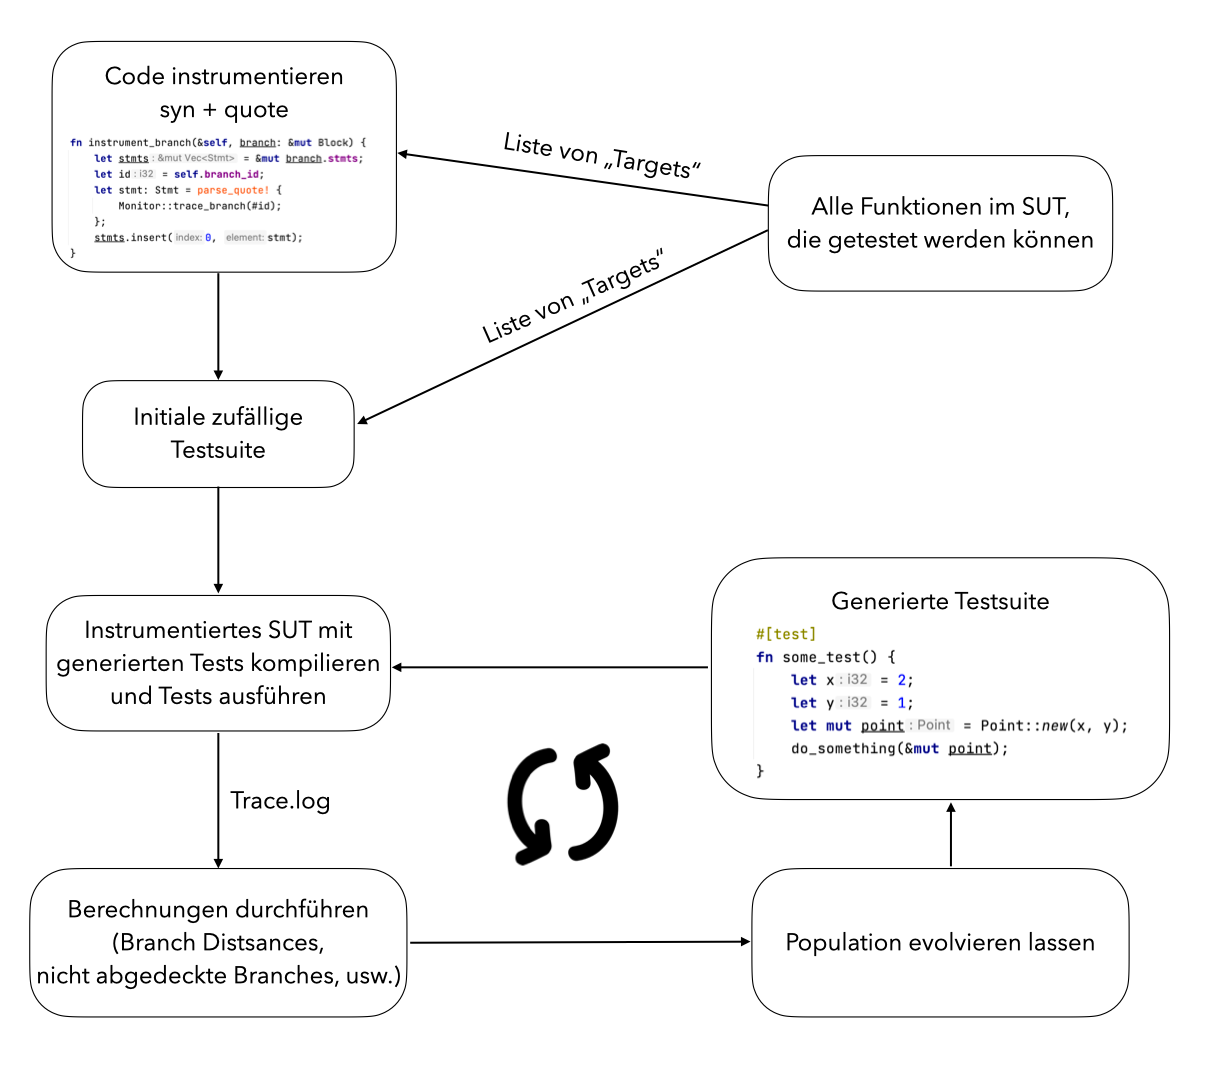
\includegraphics[width=\textwidth]{testify-overview}
\label{fig:testify-overview}
\end{figure}
\subsection{Testability Transformations}
\subsection{Instrumentation}
\subsection{Test Suite Optimization}
Figure~\cref{fig:testify-overview} illustrates the main steps in the Testify Tool: It starts by instrumenting the \ac{SUT} and inserting necessary statements to trace a programm execution. Then, a random test suite is generated based on the \ac{SUT} and evolved using evolutionary search towards a specified fitness goal. At the end, the test suite with the highest coverage is returned. 

\subsubsection{Problem representation}
Laut McMinn~\cite{McMinn_2004} sollte eine Enkodierung der Lösung so gewählt sein, dass ähnliche Lösungen ebenfalls \"Nachbarn\" im repräsentierten Suchraum sind. Dadurch kann die Suche leicht von einer zur ähnlichen Lösung durch einfache Modifikationen der Repräsentation fortgeführt werden. In genetischen Algorithmen für Testgenerierung repräsentiert ein Chromosom in einer Population typischerweise eine ganze Testuite~\cite{Fraser_2011, Campos2017}. Fraser und Arcuri schlagen folgendes zu Repräsentation der Lösung vor~\cite{Fraser_2011}: Eine Lösung ist hier eine Test Suite~$T$, die im Grunde ein Set von Unit Tests ist und für welchen gilt: Wenn~$|T| = n$, dann~$T = \{t_1, t_2, ... ,t_n\}$. 

Ein Unit Test ist demnach eine Sequenz von Statements bzw. Programmaufrufen, die Teile des \ac{SUT} ausführen, um ein gewisses Objective (bzw. Branch) zu erreichen und abzudecken. Jedes Statement ist ein Wert~$v(s_i)$, welcher von einem der fünf folgenden Typen~$\tau(v(s_i))$ sein kann:
\begin{itemize} 
	\item \textbf{Primitive Statements} repräsentieren numerische Variablen, z. B. \lstinline{let v = 42}. Der Wert und Typ des Statements werden von der primitiven Variable bestimmt. 
	\item \textbf{Konstruktor-Statements} generieren neue Instanzen eines gegebenen Structs, z. B. \lstinline{let s = SomeStruct::new()}. Der Wert und Typ des Statements werden vom Struct bestimmt. Ein Konstruktor kann Parameter haben, denen ebenso der Wert aus dem Set~$\{v(s_k) | 0 \leq k < i\}$ zugewiesen wird.
	\item \textbf{Attribut-Statements} greifen auf die public member variables von Objekten, z. B. \lstinline{let b = a.x}. Der Wert und Typ eines Attribut-Statements sind von der member variable abhängig. Die Quelle der member variable, also~\lstinline{a}, muss ebenso Teil des Sets~$\{v(s_k) | 0 \leq k < i\}$ sein. 
	\item \textbf{Methoden-Statements} führen Methoden auf Objekten aus oder rufen statische Methoden auf, z. B. \lstinline{let b = a.len()}. Hier wieder, das Quellobjekt und jegliche Parameter der Methode müssen Teil des Sets~$\{v(s_k) | 0 \leq k < i\}$ sein. Der Wert und Typ des Statements werden vom Return-Wert der Methode bestimmt. 
	\item \textbf{Funktionen-Statements} führen lose bzw. frei stehende Funktionen aus, z. B. \lstinline{let a = do_something()}. Die möglichen Parameter einer solchen Funktion müssen Teil des Sets~$\{v(s_k) | 0 \leq k < i\}$ sein. Der Wert und Typ des Statements werden vom Return-Wert der Funktion bestimmt. 
\end{itemize}

Die Sammlung von verfügbaren Structs, deren Konstruktoren, Methoden, Felder und frei stehende Funktionen sind ein sogenannter Test Cluster~\cite{Fraser_2011}. Die Größe einer Test Suite sowie einzelner Tests ist dabei dynamisch und kann sich (fast) beliebig verändern. Da für die meisten generierten Tests keine Testorakel zur Verfügung stehen werden, soll die Größe der Test Suite sowie der einzelnen Tests eine Obergrenze haben (kein Mensch möchte tausende Zeilen lange Tests durchlesen, um am Ende eine passende Assertion zu überlegen).

\subsubsection{Fitness Function}
Eine gute Fitnessfunktion ist sehr wichtig bei der Suche nach Lösungen. Lösungen, die in einer bestimmten Weise \"besser\" als andere sind, sollen mit besseren Fitnesswerten belohnt werden. Was auch immer eine bessere Fitness ist, eine höhere oder niedrigere Fitness hängt davon ab, ob die Suchstrategie versucht, die Fitnessfunktion zu maximieren oder zu minimieren~\cite{McMinn_2004}. Dieser Ansatz wird sich voraussichtlich auf Branch Coverage konzentieren. EvoSuite instrumentiert in der originalen Implementierung Java SUT auf Bytecode-Level und im Bytecode werden alle Loops usw. in die einfachen if-Verzweigungen überführt. Das Ziel ist es, die optimale Lösung zu finden, d. h. eine Test Suite, die möglichst hohe Branch-Coverage hat. Gleichzeitig soll es aber keine andere Testsuite geben, die bei gleicher Branch-Coverage kleiner ist bzw. kleinere Tests enthält. Einige Branches, sogenannte infeasible Branches, können evtl. gar nicht abgedeckt werden, entweder aufgrund der limitierten Repräsentation der Lösung oder weil es keine passenden Inputs existieren. Somit werden solche Tests bevorzugt bei der Evolvierung bevorzugt, die eine höhere Fitness bzgl. der Branch-Coverage haben. Bei zwei Tests mit der gleichen Coverage wird der kürzere bevorzugt. 

Um die Suche voranzutreiben, können verschiedene Heuristiken verwendet werden. \todo{Welche gibt es überhaupt?} Eine der weitverbreitesten ist Branch Distance. McMinn~\cite{McMinn_2004} beschreibt eine Sammlung von Regeln, die rekursiv angewendet werden können, um Distanz bei allen möglichen Prädikaten zu berechnen. Wenn die Ausführung des \ac{SUT} bei gegebenen Inputdaten in einem bestimmten Branch landet, so kann eine lokale Suche angewendet werden. Es wird mit Hilfe einer lokalen Fitnessfunktion abgeleitet, wie nah das Prädikat zum Auswerten zu \lstinline{true} ist. Zum Beispiel, bei einem Prädikat~\lstinline{x >= 10} und~\lstinline{x = 5} (während der Ausführung) wird der \lstinline{false} Branch getroffen. Die Distanz zum \lstinline{true} Branch beträge somit~$10 - 5 + k$ mit~$k \geq 1$. Dabei wird jedes Prädikat im \ac{SUT} instrumentiert, um die Distanzen zu anderen Branches während der Ausführung des \ac{SUT} zu tracen. Die Branch-Distanz muss noch normalisiert werden (je nach Werten kann es schnell zu Extremen kommen). Arcuri~\cite{Arcuri_2011} beschreibt in seiner Arbeit, welchen Einfluss die Normalisierung der Branch-Distanz auf die Effektivität einer such-basierten Testgenerierung hat. 


\subsubsection{Bloat Control}
Hier wird beschrieben, wie man verhindern kann, dass die Größe der Test Suite und einzelner Tests ausartet. Fraser und Arcuri~\cite{Fraser_2011} haben ein paar Gedanken dazu. 

\subsubsection{Search Operators}
Suchoperatoren wie Crossover, Mutation und Random Test Case werden hier beschrieben. Natürlich haben auch Fraser und Arcuri~\cite{Fraser_2011} eine ausführliche Beschreibung der Funktionsweise. 

\subsection{Usability}
EvoSuite scheint sehr auf Usability ausgerichtet zu sein, zum Beispiel gibt es ein Eclipse Plugin, welches man per Click zum Generieren von Tests für das offene Projekt benutzen kann. Außerdem, da SBST mit Iterationen arbeitet, kann man die Ausführung jederzeit beenden und die bisher besten Ergebnisse zurück geben~\cite{Harman2015}. Das obere Limit für die Ausführungszeit von generierten Tests ist in diesem Kontext von Bedeutung. 
\section{Evaluation}
\subsection{Setup}
\subsection{Threats to Validity}
\subsection{Code Coverage Comparison with Manually Written Tests}
\subsection{Code Coverage Comparison with Other Tools}


\section{Conclusion}

\section{Future Work}

\appendix
\chapter{Acronyms}
\begin{acronym}
	\acro{SUT}{System Under Test}
	\acro{CUT}{Class Under Test}
	\acro{MUT}{Method Under Test}
	\acro{SMT}{Satisfiability Modulo Theories}
	\acro{GA}{Genetic Algorithm}
	\acro{EA}{Evolutionary Algorithm}
	\acro{MOSA}{Many-Objective Sorting Algorithm}
	\acro{DynaMOSA}{Many-Objective Sorting Algorithm with Dynamic target selection}
	\acro{WS}{Whole Suite}
	\acro{WSA}{Whole Suite with Archive}
	\acro{SBST}{Search-based Software Testing}
	\acro{SBSE}{Search-based Software Engineering}
	\acro{ATP}{Automated Theorem Prover}
	\acro{DSE}{Dynamic Symbolic Execution}
	\acro{IR}{Intermediate Representation}
	\acro{MOA}{Multi- and Many-Objective Algorithm}
	\acro{DDG}{Data Dependence Graph}
	\acro{HIR}{High-level Intermediate Representation}
	\acro{THIR}{Typed HIR}
	\acro{MIR}{Mid-level Intermediate Representation}
	\acro{AST}{Abstract Syntax Tree}
	\acro{CFG}{Control Flow Graph}
	\acro{CDG}{Control Dependence Graph}
	\acro{API}{Application Programming Interface}
	\acro{NSGA-II}{Non-dominated Sorting Genetic Algorithm II}
	\acro{TCP}{Transmission Control Protocol}
	\acro{SSA}{Static Single Assignment}
\end{acronym}


\bibliographystyle{unsrt}
\bibliography{bibliography}
%\nocite*{}
\end{document}